%************************************************
\chapter{Background estimation}
\label{ch:BG}
%************************************************

The charge flip background and the fake lepton background are the two dominant backgrounds that their original particles in the final state come from the SM, but not the SUSY signal. Because of the mis-reconstruction, they pass the selections of the SRs. This type of background will be estimated by using the data-driven method.

\section{charge flip background}
\subsection{Sources for charge flip background}
The charge flip background is due to the mis-identification of the sign of the charge of a lepton, after the reconstruction.
The sign of the charge is determined by the direction of the curvature of the track.
There are two main sources for the mis-identification for the direction of the curvature.

The first source is described by the figure \ref{fig:charge_flip_bremsstrahlung}.
It is the case that the lepton interacts with the material of the detector, and a photon is emitted by the process of bremsstrahlung.
The emitted photon further produces a pair of electron and positron, namely the $\gamma$ conversion.
As shown in figure \ref{fig:charge_flip_bremsstrahlung}, if the most of the energy is carried by the positron $e^{+}$ (the purple track), the direction of the curvature of the reconstructed track (the orange track) will be reversed.
Thus, the charge of the lepton is flipped.
Because the amount of this mis-identification depends on the number of hits with the detector, and hence depends on $|\eta|$ of the original track.

\begin{figure}
\centering
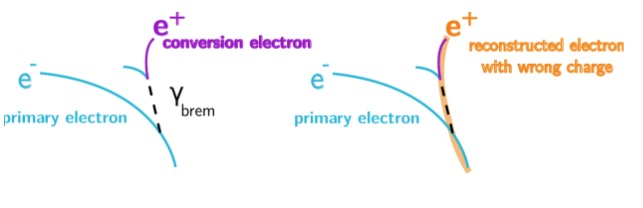
\includegraphics[width=\textwidth]{data/photo/charge_flip/Brem.jpg}
\caption{This shows how the track of the electron is incorrectly reconstructed (the orange track), due to the process of bremsstrahlung and $\gamma$ conversion.}
\label{fig:charge_flip_bremsstrahlung}
\end{figure}

The second source is described by the figure \ref{fig:charge_flip_high_pt}.
When the $p_T$ of the lepton is very high, the track of the lepton will be almost a straight line.
The curvature of the track will be close to zero, and the sign of the curvature will be difficult to distinguish.
As a result, the sign of the charge of the lepton will be incorrectly assigned.
The chance to have this problem obviously depends on $p_T$ of the lepton.

\begin{figure}
\centering
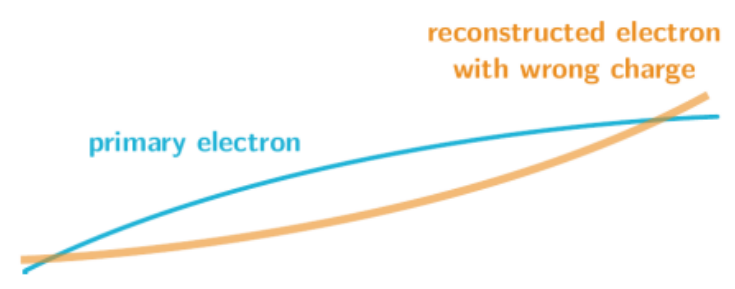
\includegraphics[width=\textwidth]{data/photo/charge_flip/WrongTrack.png}
\caption{This shows how the track of the electron is incorrectly reconstructed (the orange track), due to very high $p_T$ of the electron.}
\label{fig:charge_flip_high_pt}
\end{figure}

Compared to an electron, the charge of a reconstructed muon will be less often to be mis-identified.
The first reason is that a muon is heavier than an electron.
This will reduce the chance of the process of bremsstrahlung.
The second reason is that muons can reach to the muon spectrometer, which is the outer part of the detector, while most electrons cannot.
This means that the length of the track of a muon, which can be detected by the tracker, is longer than that of an electron.
Hence, the reconstructed curvature of the track for muons can be more accurate, and it reduces the chance of the mis-identification due to the high $p_T$.
Becasue most of the charge flip background comes from electrons, we only estimate the charge flip background for electrons.

\subsection{Likelihood method}
\label{sec:likelihood_method}
The probability that the charge of an electron is mis-identified is denoted by the charge-flip rate $\epsilon_i$, where the index i represents the dependency on the $p_T$ and $\eta$ of the electron.
The value of index i is found by splitting the variables $p_T$ and $|\eta|$ into different 2-dimensional bins, and the binning for the $p_T$ and $|\eta|$ is described by the table \ref{table:binning}. The index i of $\epsilon_i$ is defined by the index of the bin.

\begin{table}[htbp]
\centering
\begin{tabular}{|c|c|}
\hline
Variable & Boundary of the bins \\
\hline
$p_T$ (GeV) &  25, 60, 90, 130, 150, 1000 \\
\hline
$|\eta|$ & 0, 0.50, 1.00, 1.37, 1.52, 1.80, 2.00, 2.47 \\
\hline
\end{tabular}
\caption{Binning in $p_T$ and $|\eta|$ for the charge-flip rate $\epsilon_i$.}
\label{table:binning}
\end{table}

Suppose that, before the reconstruction, there are $m^{ij}_{OS}$ opposite-sign events with the leading lepton in bin $i$ and the subleading lepton in bin $j$, and similarly there are $m^{ij}_{SS}$ same-sign events.
After the reconstruction, due to the charge flip, there are $M^{ij}_{OS}$ opposite-sign events and $M^{ij}_{SS}$ same-sign events.
The number of events after the reconstruction is given by
\begin{equation}
M^{ij}_{OS} = (1-\epsilon_i) (1-\epsilon_j) m^{ij}_{OS} + \epsilon_i (1-\epsilon_j) m^{ij}_{SS} + (1-\epsilon_i) \epsilon_j m^{ij}_{SS} + \epsilon_i \epsilon_j m^{ij}_{OS} \\
\end{equation}
\begin{equation}
M^{ij}_{SS} = (1-\epsilon_i) (1-\epsilon_j) m^{ij}_{SS} + \epsilon_i (1-\epsilon_j) m^{ij}_{OS} + (1-\epsilon_i) \epsilon_j m^{ij}_{OS} + \epsilon_i \epsilon_j m^{ij}_{SS}
\label{equ:MSS}
\end{equation}
From equation \ref{equ:MSS}, the number of reconstructed same-sign events due to the real opposite-sign events, i.e. the charge flip BG , denoted by $N^{ij}_{SS}$, is
\begin{equation}
N^{ij}_{SS} = \epsilon_i (1-\epsilon_j) m^{ij}_{OS} + (1-\epsilon_i) \epsilon_j m^{ij}_{OS}
\label{equ:NSS}
\end{equation}
In the SRs, $m^{ij}_{OS}$ is the number of OS events before the reconstruction, but finally pass all selections in SRs.
$M^{ij}_{OS}$ is the total number of events that pass all selections in SRs, but replace SS requirement by OS.
Because $m^{ij}_{OS}$ is much larger than $m^{ij}_{SS}$ and the measured charge-flip rate $\epsilon_i$ is about $10^{-3}$, $m^{ij}_{OS}$ can be estimated by
\begin{align}
M^{ij}_{OS} &\approx (1-\epsilon_i) (1-\epsilon_j) m^{ij}_{OS} \\
m^{ij}_{OS} &\approx \frac{ M^{ij}_{OS} }{ (1-\epsilon_i) (1-\epsilon_j) } \\
m^{ij}_{OS} &\approx M^{ij}_{OS} \\
m^{ij}_{OS} &\approx M^{ij}_{OS} + M^{ij}_{SS}
\label{equ:mapp2}
\end{align}
By substituting equation \ref{equ:mapp2} into \ref{equ:NSS}, the charge flip BG can be estimated by $M^{ij}_{OS}$, $M^{ij}_{SS}$ and the charge-flip rate $\epsilon_i$,
\begin{align}
N^{ij}_{SS} &= \epsilon_i (1-\epsilon_j) m^{ij}_{OS} + (1-\epsilon_i) \epsilon_j m^{ij}_{OS} \\
&= [ \epsilon_i (1-\epsilon_j) + (1-\epsilon_i) \epsilon_j ] m^{ij}_{OS} \\
&\approx p_{ij} (M^{ij}_{OS} + M^{ij}_{SS}) \\
&=p_{ij} N^{ij}
\label{equ:NSS2}
\end{align}
where $p_{ij}$ and $N^{ij}$ are
\begin{align}
p_{ij} &= \epsilon_i (1-\epsilon_j) + (1-\epsilon_i) \epsilon_j \\
N^{ij} &= M^{ij}_{OS} + M^{ij}_{SS}
\end{align}
The probability density function of $N^{ij}_{SS}$, with the given values of $N^{ij}$ and $\epsilon_i$, can be described by the Poisson distribution with the mean value $\lambda = p_{ij} N^{ij}$.
\begin{align}
P(N^{ij}_{SS}|N^{ij},\epsilon_i,\epsilon_j) &= \frac{ \lambda^{N^{ij}_{SS}} e^{-\lambda} }{N^{ij}_{SS}!} \\
 &= \frac{ (p_{ij} N^{ij})^{N^{ij}_{SS}} e^{- p_{ij} N^{ij}} }{N^{ij}_{SS}!}
\label{equ:poisson}
\end{align}

In order to estimate the charge flip BG, we need to measure the charge-flip rate $\epsilon_i$.
The charge-flip rate is measured as a function of $p_T$ and $|\eta|$ by using a likelihood method, based on the 2015 and 2016 data.
A control region is used to select $Z \rightarrow ee$ processes.
Inside the control region, exactly 2 signal electrons are required.
Also, a Z mass window of 80 GeV $<m_{ll}<$100 GeV is used.
In this control region, the total number of events $N^{ij}$ and the SS events $N^{ij}_{SS}$ in each bin can be measured.
By using the equation \ref{equ:poisson}, the charge-flip rate $\epsilon_i$ can be measured by using the following likelihood method.

\section{fake lepton background}
